\documentclass[12pt,english]{article}
\usepackage{mathptmx}

\usepackage{color}
\usepackage[dvipsnames]{xcolor}
\definecolor{darkblue}{RGB}{0.,0.,139.}

\usepackage[top=1in, bottom=1in, left=1in, right=1in]{geometry}

\usepackage{amsmath}
\usepackage{amstext}
\usepackage{amssymb}
\usepackage{setspace}
\usepackage{lipsum}

\usepackage[authoryear]{natbib}
\usepackage{url}
\usepackage{booktabs}
\usepackage[flushleft]{threeparttable}
\usepackage{graphicx}
\usepackage[english]{babel}
\usepackage{pdflscape}
\usepackage[unicode=true,pdfusetitle,
 bookmarks=true,bookmarksnumbered=false,bookmarksopen=false,
 breaklinks=true,pdfborder={0 0 0},backref=false,
 colorlinks,citecolor=black,filecolor=black,
 linkcolor=black,urlcolor=black]
 {hyperref}
\usepackage[all]{hypcap} % Links point to top of image, builds on hyperref
\usepackage{breakurl}    % Allows urls to wrap, including hyperref

\linespread{2}

\begin{document}

\begin{singlespace}
\title{Impact of Donations at FBS Division 1 Universitiesl\thanks{Thank you, Prof. Ransom, for pushing my need for learning in a new direction and give me the tools to discover insight in data}}
\end{singlespace}

\author{Megan N. Yarberry \thanks{Department of Health \& Exercise Science, Sports Data Analytics Lab, University of Oklahoma.\
E-mail~address:~\href{mailto:megan.n.yarberry@ou.edu}{megan.n.yarberry@ou.edu}}}

\date{May 4, 2020}

\maketitle

\begin{abstract}
\begin{singlespace}
With over 130 teams competing in the Division I Football Bowl Subdivision every year the stakes are high and even higher for top bowls including those that are playing for a chance for the National Title. Total expenses for top teams competing for that championship grow exponentially throughout the decades and athletic departments rely heavily upon help from donors and athletic boosters to help make up the difference. Through this study is an analysis of the 2018-2019 total revenue generated by the Athletic Department and if there is a correlation between the dollar amount obtained and spent on the football team and on-field performance. Using a linear regression model to help predict total revenue and expenses spent on the football program and the seasons winning percentage. Knowing revenue is a key component to winning, exactly what is the key dollar amount might a team need to fundraise to win an NCAA Division I National Championship? 
\end{singlespace}

\end{abstract}
\vfill{}



\pagebreak{}


\section{Introduction}\label{sec:intro}
Having athletic programs in colleges gives many students an opportunity outside of the classroom to learn, grow and succeed. In 2019 the NCAA celebrated over 150 years of football and from there the sports and programs have expanded \citep{Parlier}. Over 1,200 colleges and universities across the United States have sports teams that compete through the National College Athletic Association (NCAA) on all three divisions \citep{Ncaa_2019}. 

To have sports teams compete at a high level is an expensive expenditure and it was reported in the 2018 NCAA Division I Revenues and Expense findings that the mean expenses outweighed the revenue generated \citep{Parlier}. Many schools even at the highest level of competition are running a deficit, and the deficit is then accounted for by the school. Only a handful of top-ranked schools from the major five conferences are running on a surplus of revenue \citep{Thomas}.

Revenue that is generated is primarily coming from ticket sales, marketing, broadcasting rights, and a small proportion from conference distribution \citep{Thomas}. Most revenue that is obtained is coming from largely watched sports such as football, men’s and women’s basketball, and in some cases men’s ice hockey (REF). To differentiate college at the division one level the NCAA breaks it down by if a school has a football team or not if they do, they separate them by how they compete for either the football Championship Subdivision (FCS) or schools that are Football Bowl Subdivision (FBS). Large schools that compete at the FBS can even be broken down further as to if the department runs autonomously from the University. 

Having a football team competing in the FBS is an expensive financial responsibility, with the median total expenses a department endures in one year being 115 million dollars \citep{Powell}. Universities are only contributing less than five percent of the total revenue knowing athletics departments are sometimes running a deficit \citep{Powell}. Many universities rely on supplementary revenue generators such as donors and alumni to give gifts back to the university to help their student-athletes succeed on the field and in the classroom. Gifts to the athletic department from donors are a major factor financially on running an athletic department, these gifts make up on average around twenty-four percent of the revenue an athletic department might make a year \citep{Powell}. 

Fundraising is an important key to keeping athletic departments successful and afloat financially. Many universities across the country are charging a mandatory seat donation in addition to the ticket price for season ticket holders and depending on the location is how much the addition donation is required. By giving this minimum “seat” donation numerous Universities allow you automatically join their society of donors. Through this club they offer incentive to pledge larger gifts to their programs with extra benefits to seating priority, Game Day tailgates, priority to away games tickets and exclusive content of the program’s teams. It was noted in one study that the second largest season why donors donated back to the athletic program was around ticking and seat location \citep{Gladden}. Creating this need to not only get members to renew yearly but to increase members to pledge more than the previous year but enticing members with better allocated season ticket seating.

Directors within the donor club at the University market to their members with emails, phone calls, newsletters, social media and old fashion mail. Lots of time and resources are poured in their members to create renewals and a better atmosphere fans at the college games. If directors were able to know the exact dollar amount that was needed to be donated a year to have a successful football season, would this ultimately  be helpful in the giving season? 


\section{Literature Review}\label{sec:litreview}
Athletic programs that compete in the FBS and have football teams at the Division 1-A level and are a part of one of the top five conferences, must generate a lot of revenue to be able to keep up and compete with other teams in their conference. Revenue is a large contributing factor to a successful program and success on the field during conferences and post-season bowl games. Athletic programs generate a majority of their revenue through donations from either alumni or non-alumni. These major gifts not only impact the program and the team but have a contribution to academic success and graduation rates in the classroom setting. 
\subsection{Impact of Winning Programs}
It is not a myth that having a winning FBS football program apart from your athletic department can change a University. For a university as a whole having a successful football program can attribute to higher enrolment and applicants the following school year \citep{Baumer}. Higher applicants to a University allow for larger enrollment of the incoming freshman class and an overall increase in revenue for the institution. Having a football team with an increase in win percentage will result in an increase in applicants by 1.1 percent while having a basketball team at the division one level win the National title two years prior will result in a 10 percent increase in applicants to the University \citep{Baumer}. \citet{Baumer} collected data from all 65 schools that compete in Division I football and are a part of the top five conferences, from 2015-2016 including three years in lag. This study was looking at the success of both football and men’s basketball and their impact on the institution on the academic and enrollment side.

Looking at graduation rates with the variables of success from both football and men’s basketball, proving there is a correlation between graduate rates increasing based on the performance of the football program at Division 1 programs. To come to this conclusion, data was pulled from 78 of the top teams in the country coming from the top major conferences and Universities one might choose when applying to schools with football and basketball programs. Looking at the correlation between team winning percentage, bowl appearance, and Final Four appearance does affect graduation rates \citep{Tucker}. If a 10 percent increase in winning for the football team over six years will result in a 2.1 increase in the graduation rate at the university along with a bowl game appearance increases by 1.7 percent and every bowl game after that in those six years \citep{Tucker}. 

\subsection{Cost of a Successful Program}
Having a successful program does come at a high cost and create a steep financial burden for many institutions and programs. With not all conferences having automatic bids to the FBS it becomes even more difficult for lower-level teams to compete for a spot within a bowl due to the level of competition and funding \citep{Caro}. \citet{Caro} looked at the revenue from all 120 schools that compete in the FBS looking at the 2010 season and using 2003-2009 as the dependent variables to compare too. The gap between the top five power conferences and the rest of the schools competing in the FBS is well over 20 million dollars in revenue a year, proving there is a strong correlation between conference and revenue generated \citep{Caro}. Schools that have paid top dollar to hire coaches, invest in the program and facilities are seeing the payout in bowl games which as a result has led to fans and donors following the support of a successful program.

After looking at the Caro and Benton study, the next thing was to look at a forecasted model of revenue an athletic department might generate. Knowing that the football team performance contributes a large portion of the variability to the equation. Most athletic programs run like a non-profit organization generation expenses at the same rate they are pulling in revenue \citep{Mcevoy}. \citet{Mcevoy} investigate all 120 schools that are apart of Division I FBS programs from 2002 to 2007. From this study, it was depicted that there is a strong correlation between revenue an athletic department generated and the number of varsity sports within the department and the number of student athletics apart of the University \citep{Mcevoy}. With no written correlation to why this is being contributed as a correction besides that having more athletic programs results in higher success in other programs and can create more recognition on a multi-sport platform. This study did a very basic analysis with data open to the public and does not prove much insight into why but a basic correlation.

Investing in college football is crucial for not only an increase in winning but for the student body, campus life and impact on the overall university. From these studies, there is proof in investing in college football not only to create the college experience but also increases application rates and overall student body enrollment. From having an increase in numbers students are more likely to stay on campus and partake in extracurricular activities such as support the basketball and football team, by having successful teams there is a higher chance for the student population to graduate, a correlation to increase graduation rates.

\section{Data}\label{sec:data}
The data set is looking at all 130 teams that compete at the D1 FBS level from the 2019-2020 season. The main focus is to look at what the overall impact of donations on a teams success rate at a college institution. Based off the knowledge provided by the NCAA Football programs generate the most revenue and expenses for athletic departments across the country.  

This study will look at major variables such as coaching salaries total dollar amount allocated just to the football team, total revenue and expense for the athletic department along with overall winning percentage.
The study will be looking at total revenue and expenses since the number of total donations is not public record to be analyzed. The primary source of data is coming from USA Today College Sports Database, were coaches salaries and total revenue and expenses were scrapped. A visual depiction of the deviation of total revenue generated by each school in the conference can be viewed by figure \ref{fig:fig1}. The finances in athletic departments was sites for the 2018-2019 academic school year season on USA Today by \citet{Berkowitz}. Table \ref{Table:Table1} contains summary statistics.

\citet{Berkowitz} also contributed the 2019 FBS Division I Head Coach football salaries from USA Today Sports. This data set included assistance pay, head coach total pay and bonuses paid in the 2018 season. Table \ref{Table:Table2} contains summary statistics.
My final data set came from Sports Reference for the 2018-2019 season along with the 2019-2020 season \cite{Sports2018} and \cite{Sports2019}. This website allowed for the study to scrap the number of wins and loses to create an overall percentage of success for the season. 

One of the limitations of the data set is that a few of the Universities were pulled for the 130 variables due to lack of information, many of the private institutions do not have to report financial data to the public and as a result this data was removed from the study. Along with not having the direct correlation of data coming from donation variables. A mock variable was created at the end of study to simulate the average donation amount reported by the NCAA, with this amount similar to the total revenue and each amount different for all Universities the outcome of the study did not change. 



\section{Empirical Methods}\label{sec:methods}
The goal of this study is to look for correlation between donations which results in an increase total revenue generated and on-field performance. While my approach explores a number of different approaches, the primary empirical model can be depicted in the following equation:
\begin{equation}
\label{eq:1}
Y_{WinPerc}= \alpha_{} + X_{1}{Total.Revenue}+X_{2}{Total.Allocated}+X_{3}{Total.Pay}+X_{4}{Asst.Pay.Total}
\end{equation}
where $Y_{WinPerc}$ is a continuous outcome variable for the teams winning percentage $i$ in year $t$ which was done using the 2018-2019 season and 2019-2020 season. And $X_{it}$ are characteristics about $i$, which are independent of each other. These include total revenue the athlete department generated during the 2018-2019 season, total allocated dollar amount to the football team, total pay to the head coach and total pay of all football coach assistants The parameter of interest is $\alpha_{1}$.

This empirical model was also looked at looking at total expenses which is depicted through this equation: 
\begin{equation}
\label{eq:2}
Y_{WinPerc}= \alpha_{} + X_{1}{Total.Expenses}+X_{2}{Total.Allocated}+X_{3}{Total.Pay}+X_{4}{Asst.Pay.Total}
\end{equation}

Through this second equation all variables stayed the same except the first independent $X_{it}$ which was changed from total revenue the athletic department generated a year, to total expenses for the entire department not just allocated to the football team. 


\section{Research Findings}\label{sec:results}
This empirical model was run two times to see which one was more correlated with the outcome $Y_{WinPerc}$ looking at the winning percentage from the 2018/2019 and 2019/2020 season to the financial data to see if a year different had a large impact on the overall season record. Though this the 2019/2020 was statistically significant with a p-value less then .05 but the R-squared was 0.1511, reporting a weak positive correlation. Two variable found to be statistically significant was total pay of the head coach and the constant. 

The same empirical model was running changing the $Y_{WinPerc}$ to the 2018-2019 season overall win percentage. The main results are reported in Table \ref{Table:Table3}. From this table it is noted that the equation is statistically significant and the R-squared value increases from the original vale to 0.2129 creating a stronger positive correlation between revenue generated and the outcome of the FBS football season. In this new equation total revenue both variables from the 2019-2020 season results were found to be constants.

Taking the empirical model a little further and to see if there is a stronger correlation between between what type of FBS school. In a study done by \citet{Caro} looking at the financial difference between FBS conferences and generated revenue. Through the study they found that top five power conferences: Atlantic Coast Conference (ACC), Big 10, Big 12, Pacific-12 Conference (PAC-12) and Southeastern Conference (SEC), generate more than \$20 million dollars in revenue more in a season than over programs in difference conferences \citep{Caro}. Knowing this taking the study further by breaking down programs between being apart of a "Power Five" conference and those that are not. From here the study was rerun and the schools apart of the one of the power five conferences showed to have a stronger correlation with the R-squared value reaching to 0.4224. The main results are reported in Table \ref{Table:Table4}. 

In the empirical model 2, just for reference all the equations were reran to see if the data was more correlated with expenses versus revenue. In both cases for the 2018 and 2019 season data the correlation did become stronger by very few percentage points. Overall none of the equations even for the separation of "Power 5" and Non-Power 5 schools became more positive correlation due to the total dollar amount of expenses the athletic department was incurring over the year.   

With not having direct reporting of the annual donation amount and knowing the average donation amount is 24\% I rename the equation with new variables for the total revenue, and found new statistically different results then the study reported originally.


\section{Conclusion}\label{sec:conclusion}
Even though many study have proven that on-field performance those not have an impact on donation. Including this study done analyzing a decade of donation patterns from the University of Miami (FL), done by \citet{Cohen}. During which the football team won two national titles, no statistically significant data points were found \citep{Cohen}. 

The findings of this study show there a weak positive correlation between revenue generated which can be accounted for at least 24\% from donations and on team performance, there is an even stronger correlation between those teams that compete at the highest level within the "Power 5" conferences and compete for the National Title in FBS D1 Football. 

From these results and a stronger set of data it might be possible to formulate a prediction model to forecast win percentage based off revenue. Similar to to the concept of Moneyball which was formed around giving each win a dollar value. Giving athletic directors a more nominal goal campaigning for donations. Along with would these similar results be found in others ports such as basketball since there is a massive correlation between success and the impact on the study body. 

Having this correlation not only give athletic directors a more nominal goal for needed donations for a successful season it might help to correlation how much head coaches really should be paid and justify a raise or pay cut along with incentive donors with the amount they are contributing to a teams success on the field and in the classroom. A study looking at three different athletic programs across the country surveyed the schools donors that contributed to the athletic department \citep{Gladden}. From this study the number one reason which contained 61\% of the response was to help improve the success of the tam \citep{Gladden}. Knowing this from past studies what is the probability that there would be an increase in donations since it is statistically significant that the data is helping improve on-field performance for FBS "Power 5" teams, will schools see an increase in donation if this information is advertised to donors and booster for the program? 

For schools not in a "Power Five" conference would it be more realistic to set up the empirical model as a logic formula with the overall outcome being either they made it to a bowl game or not, instead of a continues winning variable that would be much more attainable then a overall winning percentage. 

\vfill
\pagebreak{}
\begin{spacing}{1}
\bibliographystyle{jpe}
\bibliography{PS11_Yarberry.bib}
\addcontentsline{toc}{section}{References}
\end{spacing}

\vfill
\pagebreak{}
\clearpage

%========================================
% FIGURES AND TABLES 
%========================================
\section*{Figures and Tables}\label{sec:figTables}
\addcontentsline{toc}{section}{Figures and Tables}
%----------------------------------------
% Figure 1 
%----------------------------------------
\begin{figure}[ht]
\centering
\bigskip{}
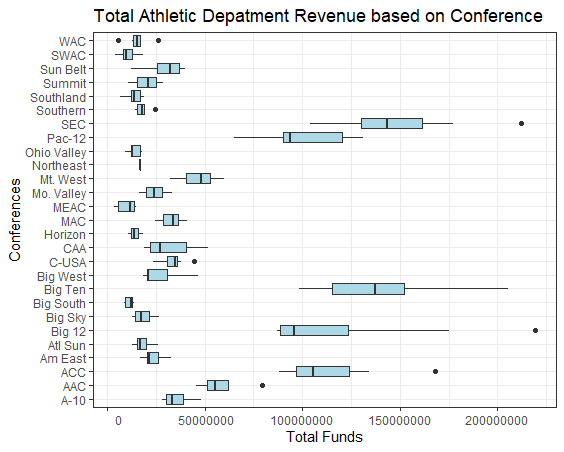
\includegraphics[width=.9\linewidth]{Image1.png}
\caption{Dispersion of total revenue generated by conference with a FBS D1 Football Team}
\label{fig:fig1}
\end{figure}
%----------------------------------------
% Table 1
%----------------------------------------
\begin{table}[!htbp] \centering 
\label{Table:Table1}
  \caption{Total Revenue and Expenses by D1 Athlete Departments in the 2018 -2019 Season} 
  \label{} 
\begin{tabular}{@{\extracolsep{5pt}}lccccccc} 
\\[-1.8ex]\hline 
\hline \\[-1.8ex] 
Statistic & \multicolumn{1}{c}{N} & \multicolumn{1}{c}{Mean} & \multicolumn{1}{c}{St. Dev.} & \multicolumn{1}{c}{Min} & \multicolumn{1}{c}{Pctl(25)} & \multicolumn{1}{c}{Pctl(75)} & \multicolumn{1}{c}{Max} \\ 
\hline \\[-1.8ex] 
Total Revenue & 230 & 47,335,695.000 & 47,754,746.000 & 3,561,797 & 14,940,098 & 55,342,752.0 & 219,402,579 \\ 
Total Expenses & 230 & 46,277,240.000 & 44,964,398.000 & 4,175,281 & 15,548,762 & 54,582,391 & 206,554,432 \\ 
Total Allocated & 230 & 12,980,065.000 & 8,709,193.000 & 0 & 7,391,702.0 & 18,706,221.0 & 41,701,756 \\ 
\hline \\[-1.8ex] 
\end{tabular} 
\end{table} 


%----------------------------------------
% Table 2
%----------------------------------------
\begin{table}[!htbp] \centering 
\label{Table:Table2}
  \caption{FBS Head Football Coach and Assistant Coach Salaries} 
  \label{} 
\begin{tabular}{@{\extracolsep{5pt}}lccccccc} 
\\[-1.8ex]\hline 
\hline \\[-1.8ex] 
Statistic & \multicolumn{1}{c}{N} & \multicolumn{1}{c}{Mean} & \multicolumn{1}{c}{St. Dev.} & \multicolumn{1}{c}{Min} & \multicolumn{1}{c}{Pctl(25)} & \multicolumn{1}{c}{Pctl(75)} & \multicolumn{1}{c}{Max} \\ 
\hline \\[-1.8ex] 
School Pay & 122 & 2,658,563.000 & 2,011,633.000 & 360,000.000 & 800,000.000 & 3,961,500.000 & 9,255,000.000 \\ 
Total Pay & 122 & 2,667,022.000 & 2,018,400.000 & 360,000.000 & 800,000.000 & 3,961,500.000 & 9,315,600.000 \\ 
Asst Pay Total & 130 & 2,445,085.000 & 2,038,775.000 & 0 & 1,035,325 & 3,769,731.0 & 7,541,277 \\ 
\hline \\[-1.8ex] 
\end{tabular} 
\end{table}

%----------------------------------------
% Table 3
%----------------------------------------
\begin{table}[!htbp] \centering 
\label{Table:Table3}
  \caption{2018-2019 Win Percentage Empirical Findings} 
  \label{} 
\begin{tabular}{@{\extracolsep{5pt}}lc} 
\\[-1.8ex]\hline 
\hline \\[-1.8ex] 
 & \multicolumn{1}{c}{\textit{Dependent variable:}} \\ 
\cline{2-2} 
\\[-1.8ex] & PCT.18 \\ 
\hline \\[-1.8ex] 
 Total.Revenue & $-$0.000 \\ 
  & (0.000) \\ 
  & \\ 
 Total.Allocated & 0.000 \\ 
  & (0.000) \\ 
  & \\ 
 Total.Pay & 0.00000$^{***}$ \\ 
  & (0.00000) \\ 
  & \\ 
 Asst.Pay.Total & 0.00000 \\ 
  & (0.00000) \\ 
  & \\ 
 Constant & 0.413$^{***}$ \\ 
  & (0.099) \\ 
  & \\ 
\hline \\[-1.8ex] 
Observations & 88 \\ 
R$^{2}$ & 0.213 \\ 
Adjusted R$^{2}$ & 0.175 \\ 
Residual Std. Error & 0.203 (df = 83) \\ 
F Statistic & 5.613$^{***}$ (df = 4; 83) \\ 
\hline 
\hline \\[-1.8ex] 
\textit{Note:}  & \multicolumn{1}{r}{$^{*}$p$<$0.1; $^{**}$p$<$0.05; $^{***}$p$<$0.01} \\ 
\end{tabular} 
\end{table} 

%----------------------------------------
% Table 4
%----------------------------------------
\begin{table}[!htbp] \centering 
\label{Table:Table4}
  \caption{Power 5 Conferences from the 2018-2019 Season} 
  \label{} 
\begin{tabular}{@{\extracolsep{5pt}}lc} 
\\[-1.8ex]\hline 
\hline \\[-1.8ex] 
 & \multicolumn{1}{c}{\textit{Dependent variable:}} \\ 
\cline{2-2} 
\\[-1.8ex] & PCT.18 \\ 
\hline \\[-1.8ex] 
 Total.Revenue & $-$0.000 \\ 
  & (0.000) \\ 
  & \\ 
 Total.Allocated & $-$0.000 \\ 
  & (0.000) \\ 
  & \\ 
 Total.Pay & 0.00000$^{***}$ \\ 
  & (0.00000) \\ 
  & \\ 
 Asst.Pay.Total & 0.00000 \\ 
  & (0.00000) \\ 
  & \\ 
 Constant & 0.249$^{**}$ \\ 
  & (0.114) \\ 
  & \\ 
\hline \\[-1.8ex] 
Observations & 49 \\ 
R$^{2}$ & 0.422 \\ 
Adjusted R$^{2}$ & 0.370 \\ 
Residual Std. Error & 0.173 (df = 44) \\ 
F Statistic & 8.044$^{***}$ (df = 4; 44) \\ 
\hline 
\hline \\[-1.8ex] 
\textit{Note:}  & \multicolumn{1}{r}{$^{*}$p$<$0.1; $^{**}$p$<$0.05; $^{***}$p$<$0.01} \\ 
\end{tabular} 
\end{table} 
\end{document}